\documentclass[12pt,a4paper,oneside]{article}

\usepackage[a4paper]{geometry}
\usepackage{amsmath,amsthm,amssymb}

\RequirePackage[utf8]{inputenc}
\RequirePackage[T1]{fontenc}
\RequirePackage{lmodern}
\RequirePackage[english]{babel}
\RequirePackage{graphicx}
\RequirePackage{scrpage2}
\RequirePackage{pifont}

\usepackage{listings}

\usepackage{hyperref}

\usepackage{graphicx}

\pagestyle{scrheadings}

\lohead{\rm Peter Brunnader}
\cohead{\rm Week 6 Assignment}
\rohead{\rm PARADIS}

\cfoot{ \arabic{page} }


\title{Week 6 Assignment \\ \normalsize Parallel and distributed programming, PARADIS \\ Department of Computer and Systems Sciences, DSV \\ Stockholm University, SU}
\author{Peter Brunnader} 
\date{\today}


\usepackage{natbib}
\usepackage[notlof,notlot,nottoc]{tocbibind}


\usepackage{fontspec}
\usepackage{xunicode}

\defaultfontfeatures{Mapping=tex-text, Ligatures=Common,
	Scale=MatchLowercase,Numbers=OldStyle}
\setmainfont{Myriad Pro}
\setsansfont{Myriad Pro}

\usepackage{color}

\definecolor{mygreen}{rgb}{0,0.6,0}
\definecolor{mygray}{rgb}{0.5,0.5,0.5}
\definecolor{mymauve}{rgb}{0.58,0,0.82}
\definecolor{gray}{rgb}{0.95,0.95,0.95}


\lstset{ %
  backgroundcolor=\color{gray},   % choose the background color; you must add \usepackage{color} or \usepackage{xcolor}
  basicstyle=\footnotesize,        % the size of the fonts that are used for the code
  breakatwhitespace=false,         % sets if automatic breaks should only happen at whitespace
  breaklines=true,                 % sets automatic line breaking
  captionpos=b,                    % sets the caption-position to bottom
  commentstyle=\color{mygreen},    % comment style
  deletekeywords={...},            % if you want to delete keywords from the given language
  escapeinside={\%*}{*)},          % if you want to add LaTeX within your code
  extendedchars=true,              % lets you use non-ASCII characters; for 8-bits encodings only, does not work with UTF-8
  frame=no,                    % adds a frame around the code
  keepspaces=true,                 % keeps spaces in text, useful for keeping indentation of code (possibly needs columns=flexible)
  keywordstyle=\color{blue},       % keyword style
  % language=Octave,                 % the language of the code
  morekeywords={*,open},            % if you want to add more keywords to the set
  numbers=left,                    % where to put the line-numbers; possible values are (none, left, right)
  numbersep=5pt,                   % how far the line-numbers are from the code
  numberstyle=\tiny\color{mygray}, % the style that is used for the line-numbers
  rulecolor=\color{black},         % if not set, the frame-color may be changed on line-breaks within not-black text (e.g. comments (green here))
  showspaces=false,                % show spaces everywhere adding particular underscores; it overrides 'showstringspaces'
  showstringspaces=false,          % underline spaces within strings only
  showtabs=false,                  % show tabs within strings adding particular underscores
  stepnumber=1,                    % the step between two line-numbers. If it's 1, each line will be numbered
  stringstyle=\color{mymauve},     % string literal style
  tabsize=2,                       % sets default tabsize to 2 spaces
  title=\lstname                   % show the filename of files included with \lstinputlisting; also try caption instead of title
}



\begin{document}
% \newgeometry{bottom=0.1cm}
\maketitle
\thispagestyle{empty}
% \def\contentsname{\empty}
% \tableofcontents
% \clearpage
% \restoregeometry
% \setcounter{page}{1}

\section{Benchmark tests: ring.erl}
I have run two benchmark test to see how and if the performance is increasing by using one core or more by using the argument \texttt{erl -smp enable} and \texttt{erl -smp disable}. My system is a MacBookAir with a 1,8 GHz Intel Core i7 CPU, so in the enabled mode 4 cores where used. \\
\\
The runtime of the \textit{parallel} executed test took basically more time, so the speedup is in general less the 1 (a deterioration). This could be that the overhead to schedule and manage is bigger than the benefit of parallelisation. But on the other hand in my opinion it is not a good example to parallelise because every process has to wait for the previous process to finish and then the next process can start to process. This is called data dependency and this is very high. \\
\\
In Figure~\ref{fig:example3} the two lines are describing the $\sum = N * M$ and $N$ is the number of processes and $\sum$ is here a constant value $8292$. In this graph you can see that  the performance is decreasing by an increasing number of processes in the case using the argument \texttt{erl -smp enable} when it comes to a number of 512 processes or nodes in the ring. \\
\\
I had a look on the use of the available cores but I have observe that more or less just two CPU where used and the total use was around 100 percent. So I would assume that two cores have alternate to do that task.
\begin{figure}[h!]
	\center
	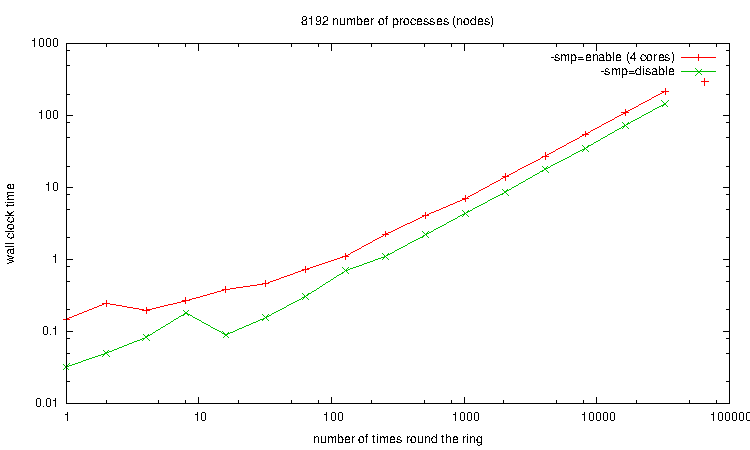
\includegraphics[width=1\textwidth]{img/8192_number_of_processes.pdf}
	\caption{Wall Clock Time by a fixed number of processes and increasing number of rounds in the ring}
    \label{fig:example1}
\end{figure}
\begin{figure}[h!]
	\center
	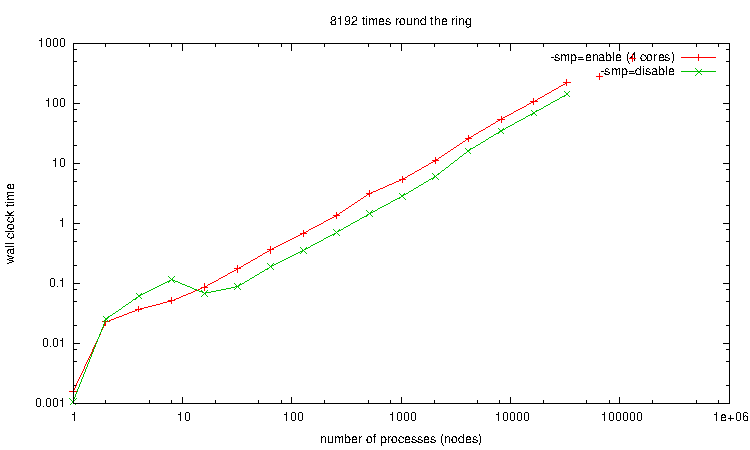
\includegraphics[width=1\textwidth]{img/8192_times_round_the_ring.pdf}
	\caption{Wall Clock Time by a fixed number of rounds and increasing number of processes}
    \label{fig:example2}
\end{figure}

\begin{figure}[h!]
	\center
	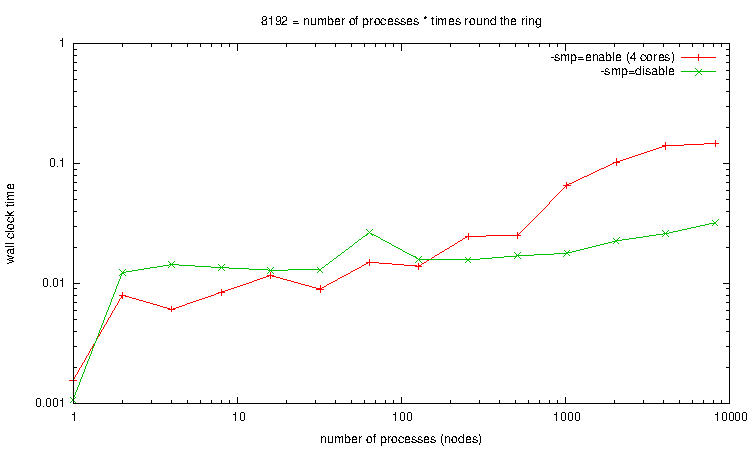
\includegraphics[width=1\textwidth]{img/8192_IS_number_x_times.pdf}
	\caption{Wall Clock Time by increasing number of processes and doing \textit{calculations} to get the sum of 8192.}
    \label{fig:example3}
\end{figure}

% \bibliographystyle{plain}
% \bibliography{literature}






\end{document}
